\chapter{How Cameras Work}

Let's say it is a sunny day and you are standing in a field a few meters
from a cow. You use the camera on your phone to take a picture of the
cow. How does that whole process work?
\index{camera}
\begin{figure}[htbp]
    \centering
    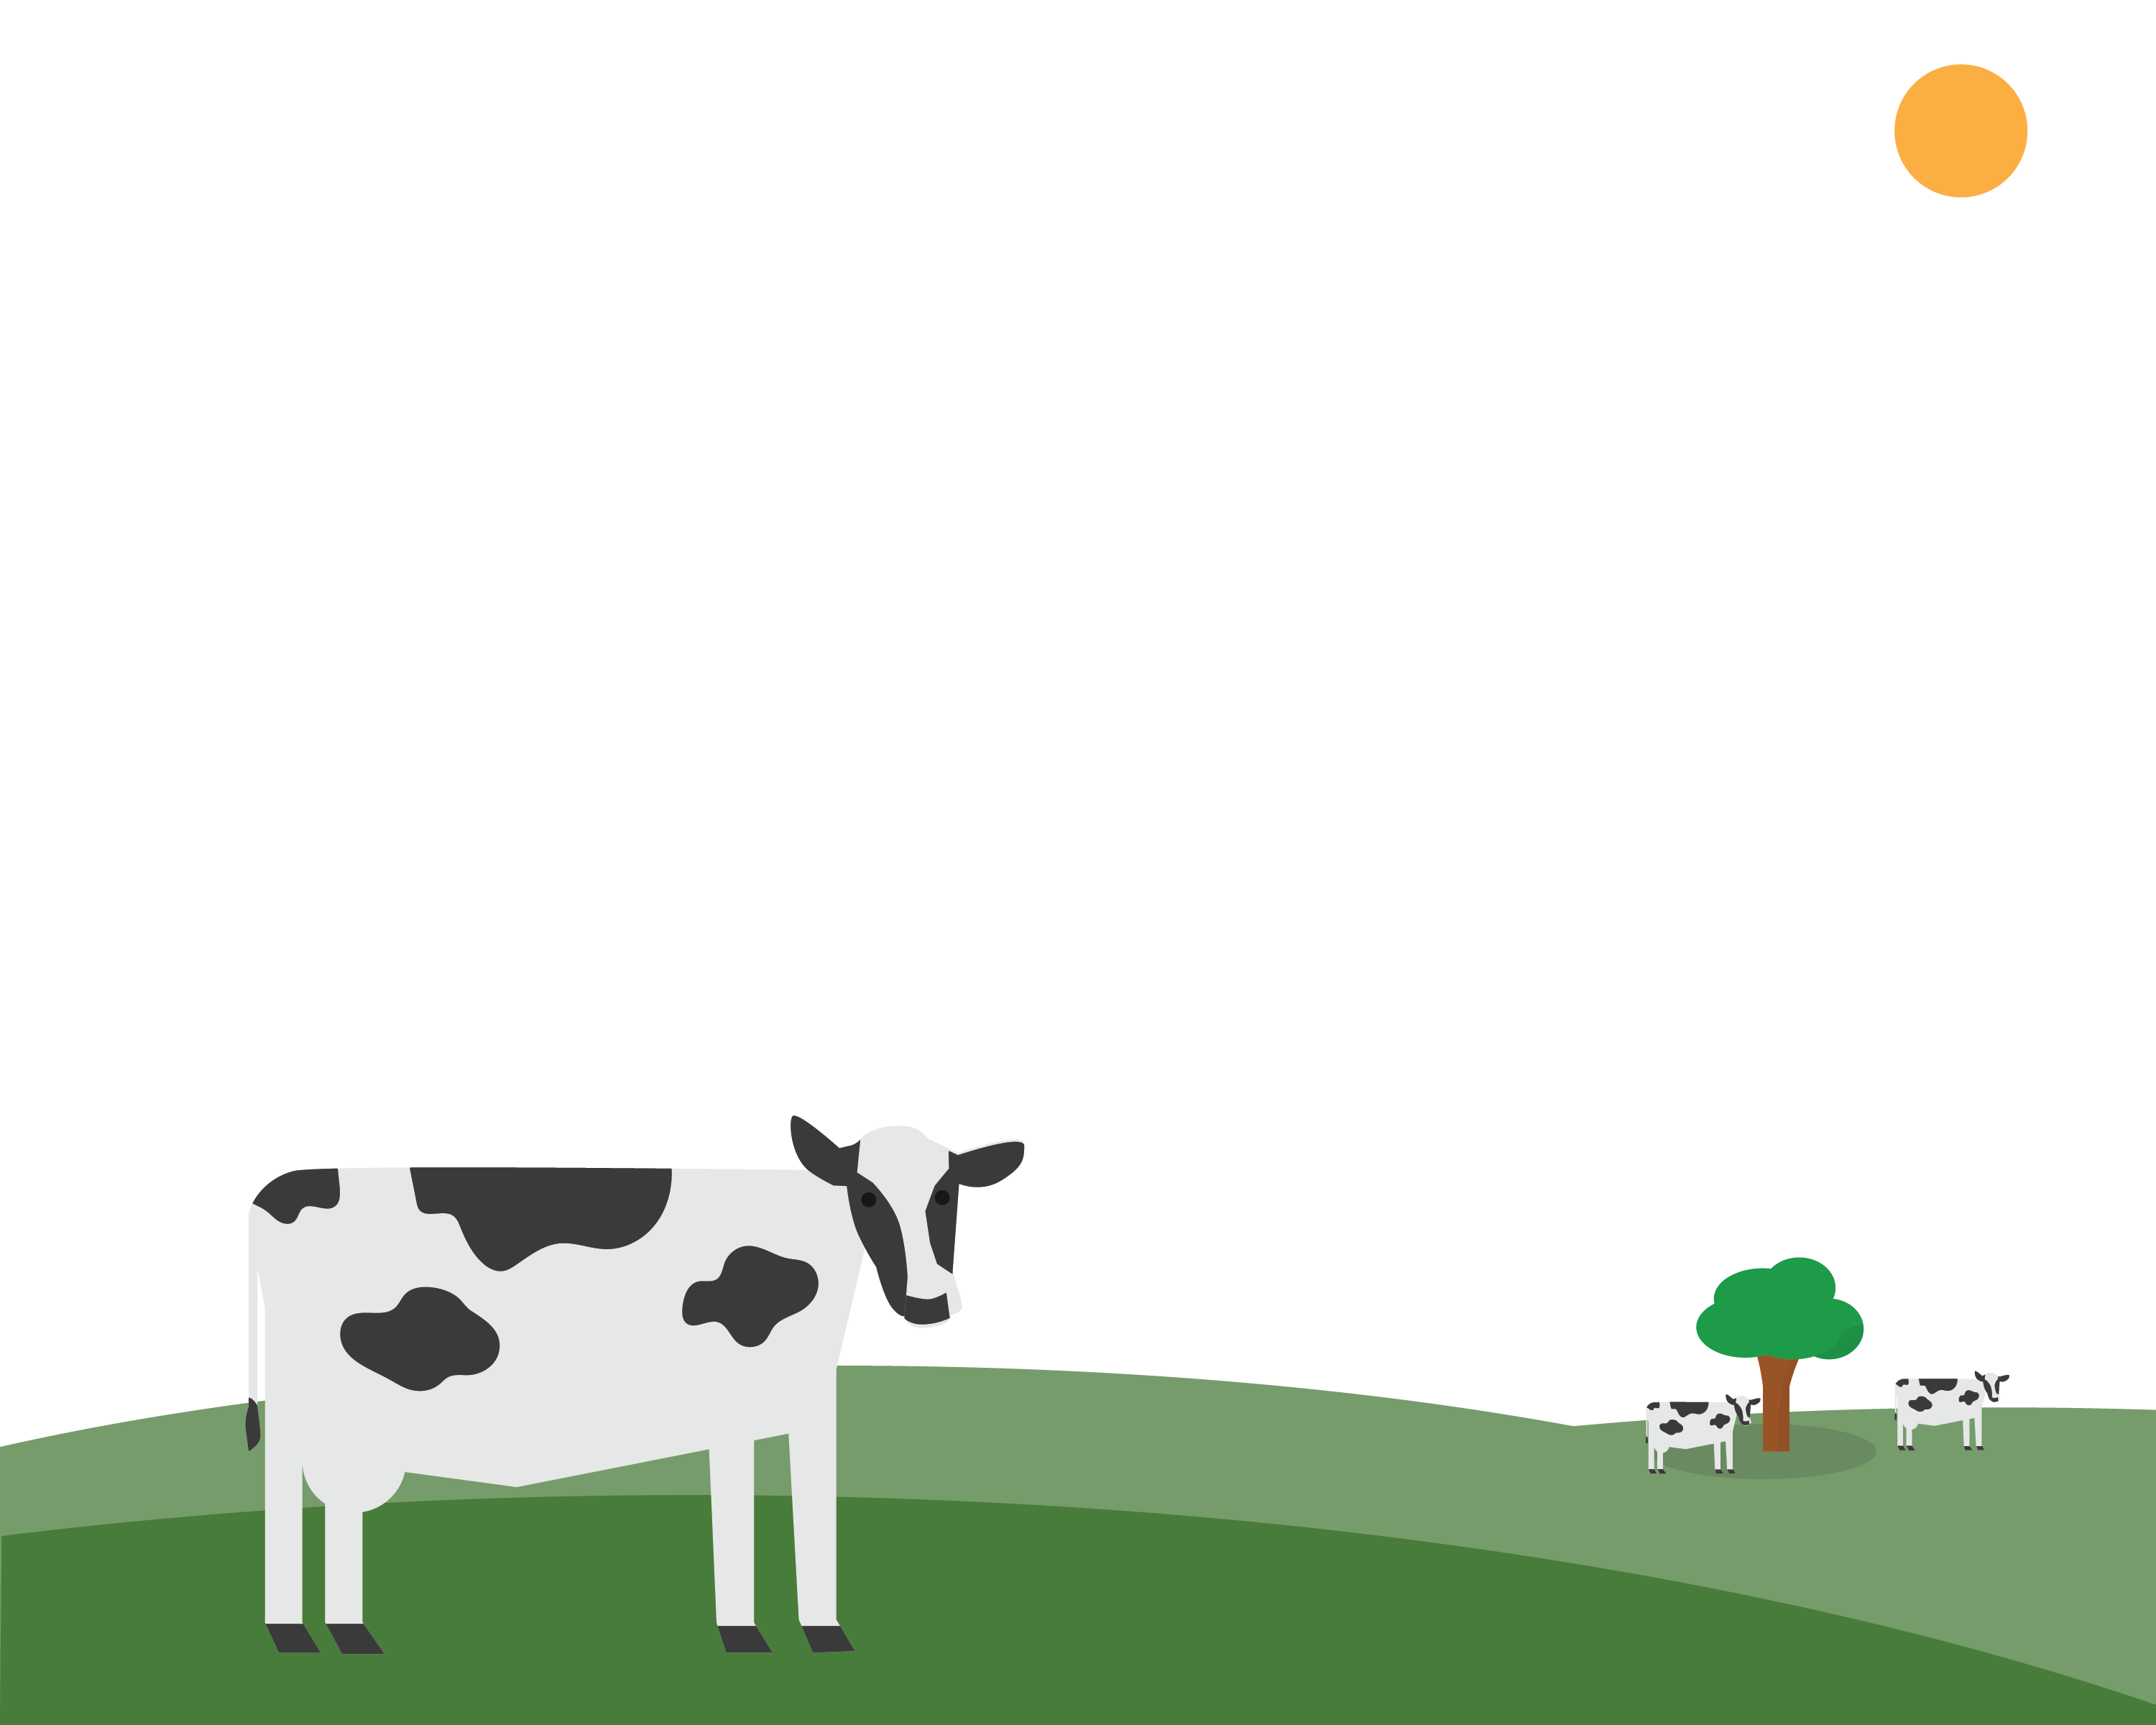
\includegraphics[width=1\textwidth]{cow1.png}
    \caption{A cow in a field.}
    \label{fig:cow1}
\end{figure}


\section{The Light That Shines On the Cow}

The sun is a sphere of hot gas. About 70\% of the gas is
hydrogen. About 28\% is helium. There's also a little carbon, nitrogen,
and oxygen.

Gradually, the sun is converting hydrogen into helium through a
process known as ``nuclear fusion'' (which we will be discussing more in a future chatper). A large amount of heat is created in this
process. This heat makes the gases glow.

\index{photon}
How does heat make things glow? The heat pushes the electrons into
higher orbitals. When they come back down to a lower orbital, they
release a photon of energy, which travels away from the atom as an
electromagnetic wave.
\begin{figure}[htbp]
    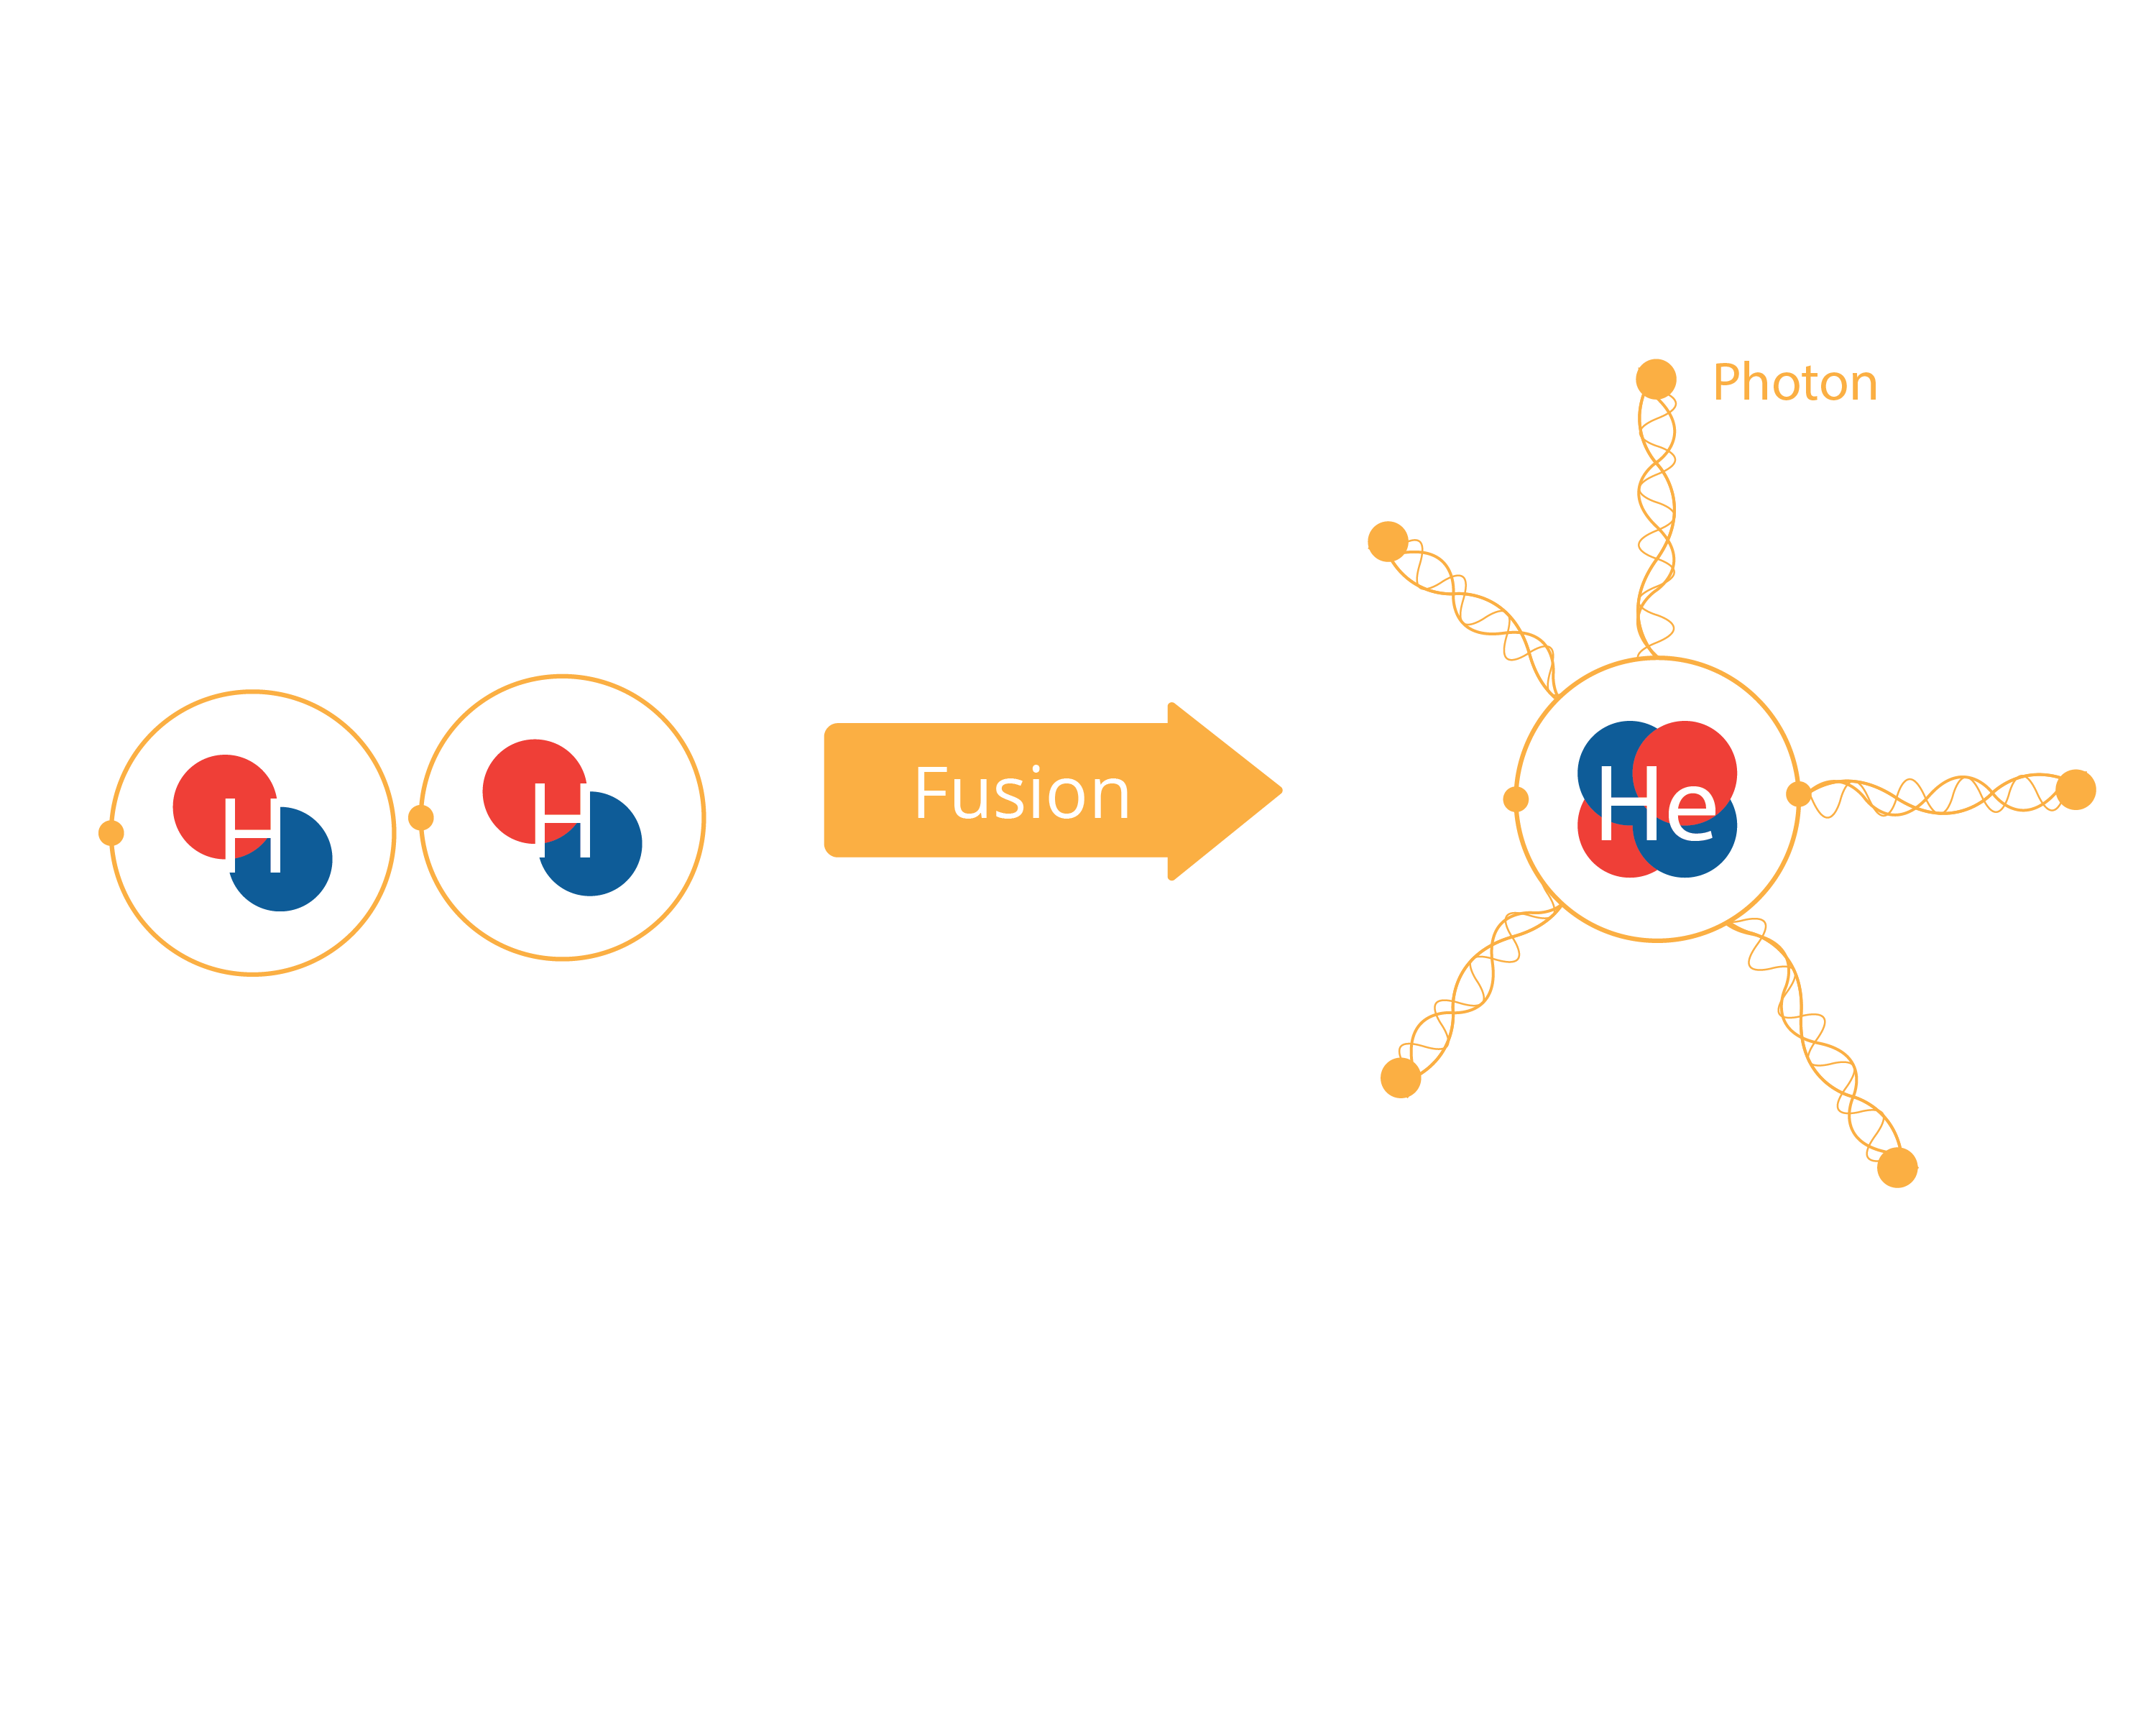
\includegraphics[width=.5\textwidth]{cow2.png}
    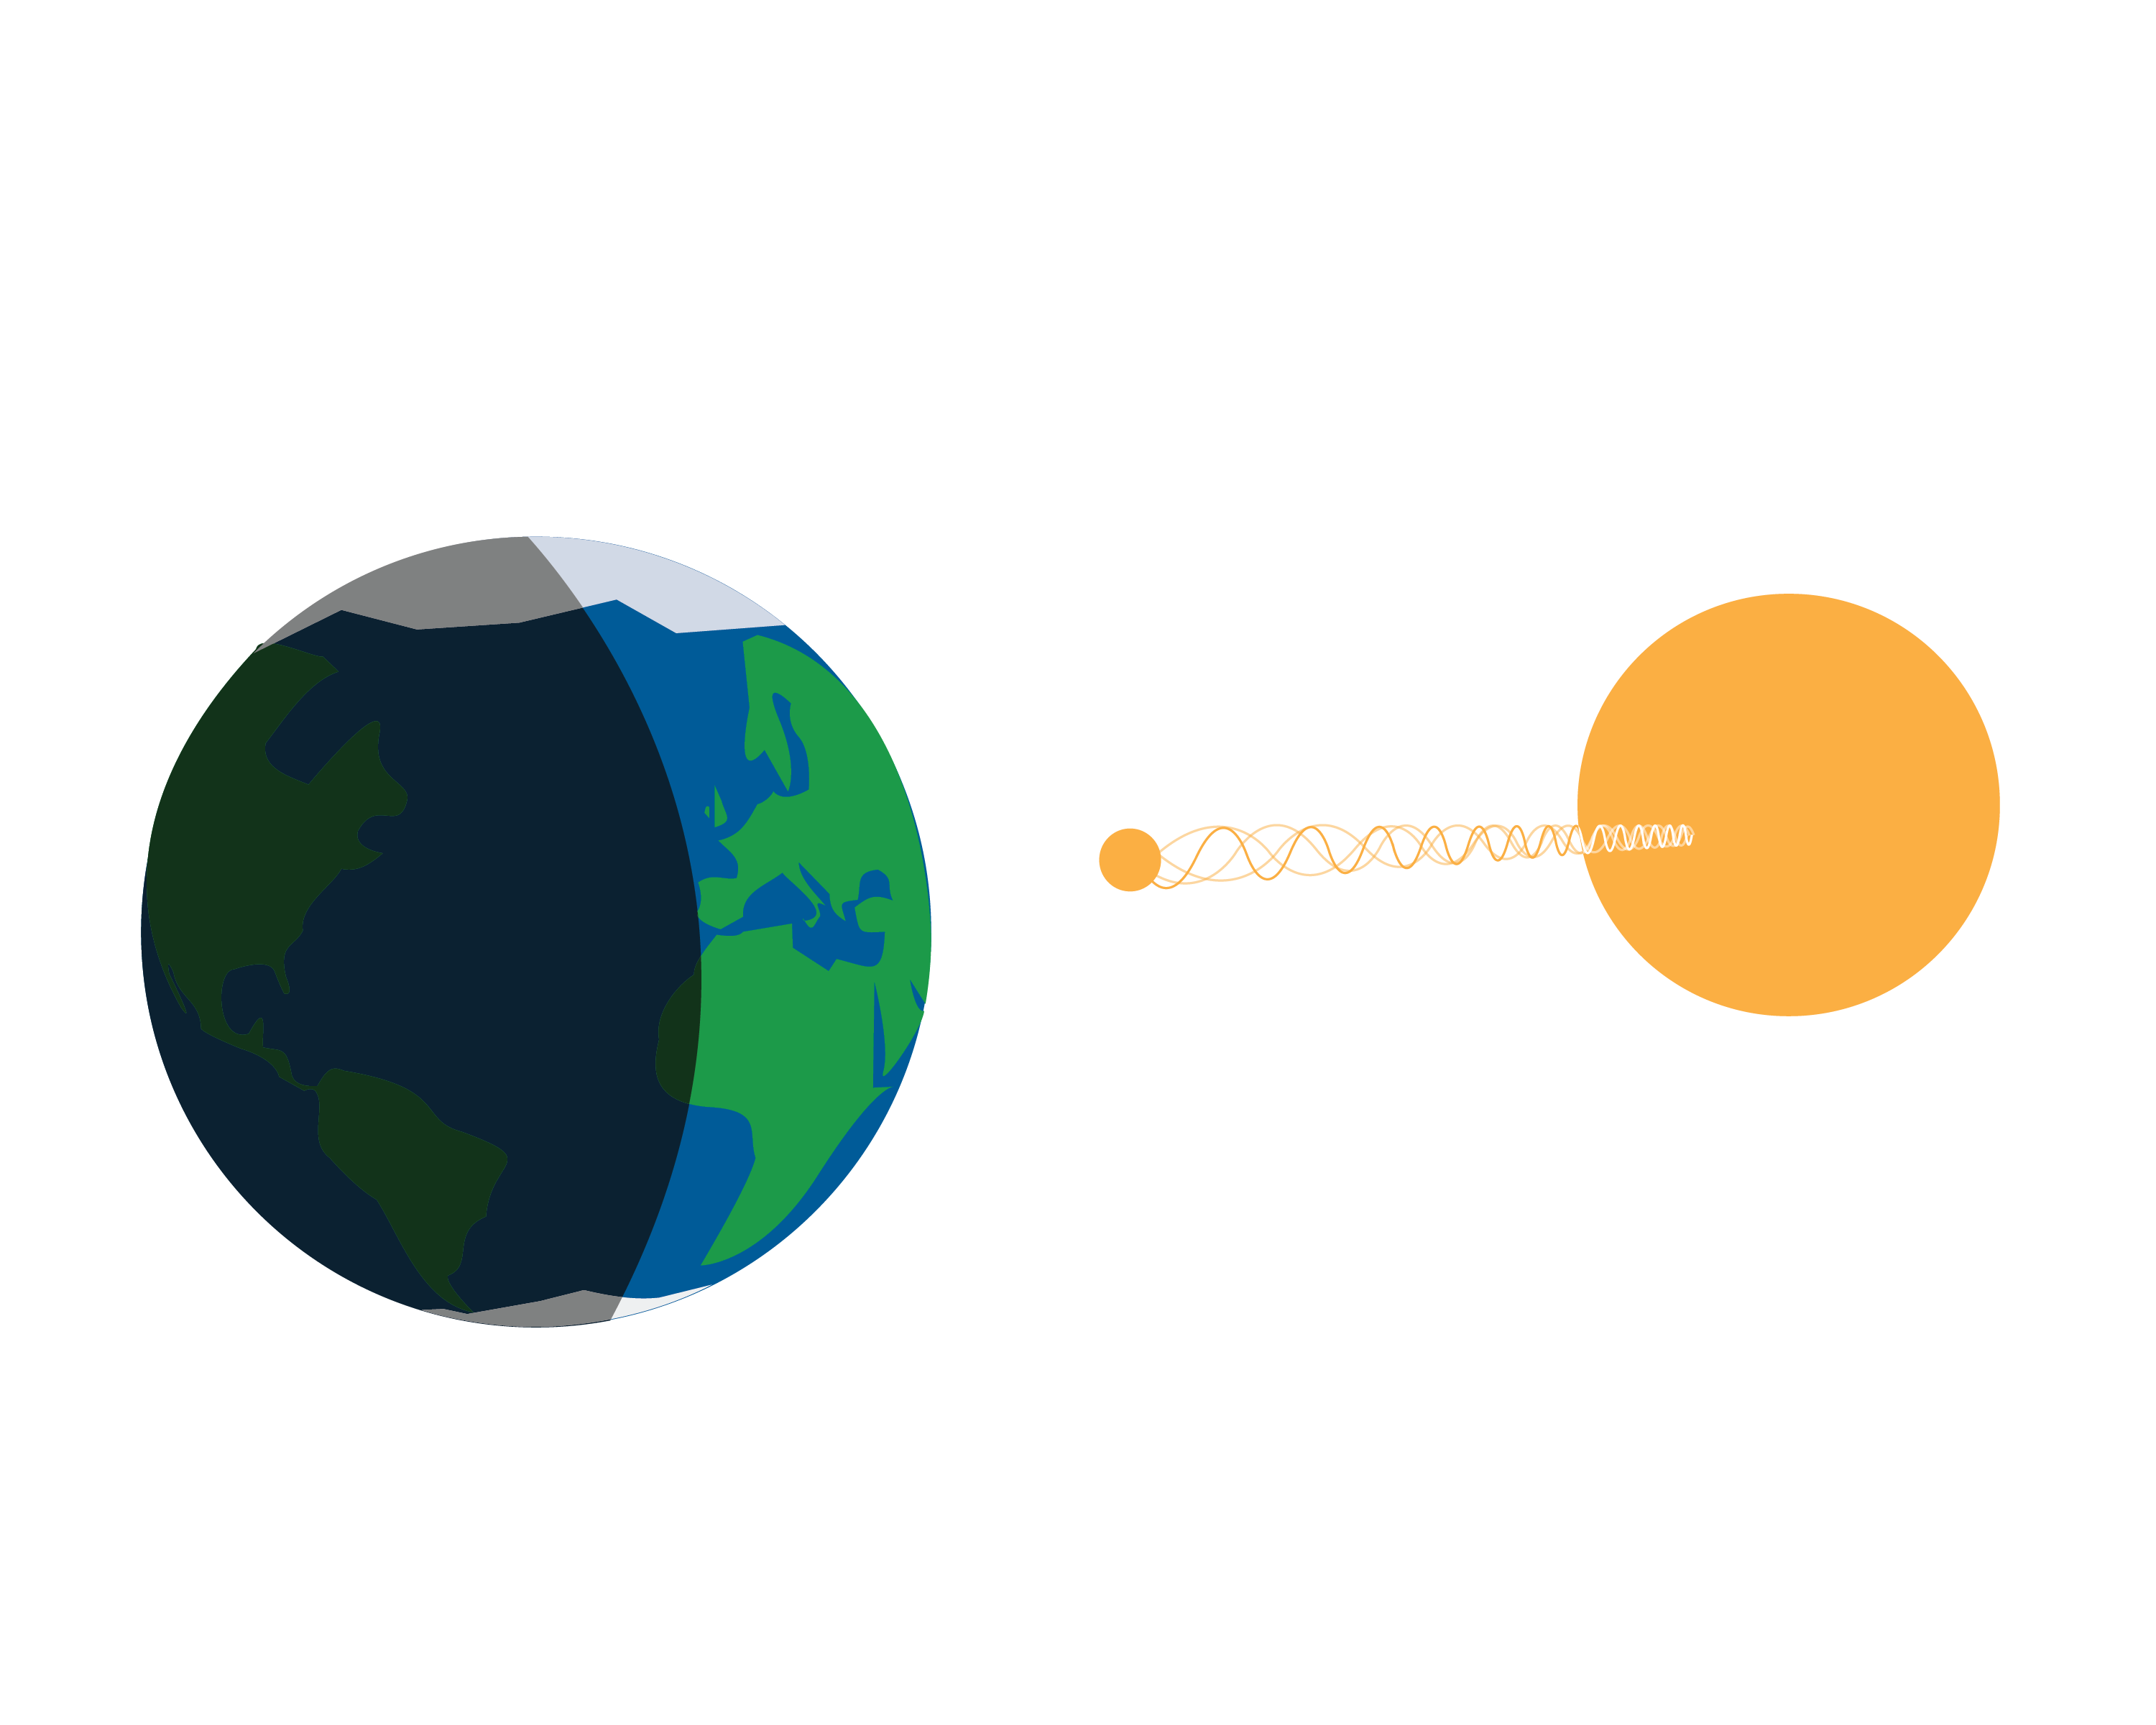
\includegraphics[width=.5\textwidth]{cow3.png}
    \caption{Photons are released when the sunlight hits the cow.}
    \label{fig:photonreleases}
\end{figure}

Heat is not the only way to push the electrons into a higher
orbital. For example, a fluorescent lightbulb is filled with gas.
When we pass electricity through the gas, its electrons are moved to a
higher orbital. When they fall back to a lower orbital, light is created.

What is the frequency of the wave that the photon travels on?
Depending on what orbital it falls from and how far it falls, the
photon created has different amounts of energy. The amount of energy
determines the frequency of the electromagnetic wave.

\begin{mdframed}[style=important, frametitle={Formula for energy of a photon}]

If you want to know the amount of energy $E$ in a photon, here is the formula:

$$E = \frac{h c}{\lambda}$$

where $c$ is the speed of light, $\lambda$ is the wavelength of the
electromagnetic wave, and $h$ Planck's constant: $6.63 \times 10^{-34} m^2 kg/s$

For example, a red laser light has a wavelength of about 630 nm. So, the energy in each photon is:

$$\frac{(300 \times 10^6) (6.63 \times 10^{-34})}{630 \times 10^{-9}} = 3.1 \times 10^{-19} \text{ joules}$$

\end{mdframed}
In the sun, there are several kinds of molecules and each has a few
different orbitals that the electrons can live in. Thus, the light
coming from the sun is made up of electromagnetic waves of many
different frequencies.

We can see some of these frequencies as different colors, but some are
invisible to humans, such as ultraviolet and infrared.

\section{Light Hits the Cow}


When these photons from the sun hit the cow, the hide and hairs of the
cow will absorb some of the photons. These photons will become heat
and make the cow feel warm. Some of the photons will not be absorbed
-- they will leave the cow. When you say ``I see the cow,'' what you are
really saying is ``I see some photons that were not absorbed by the cow.''

\begin{figure}[htbp]
    \centering
    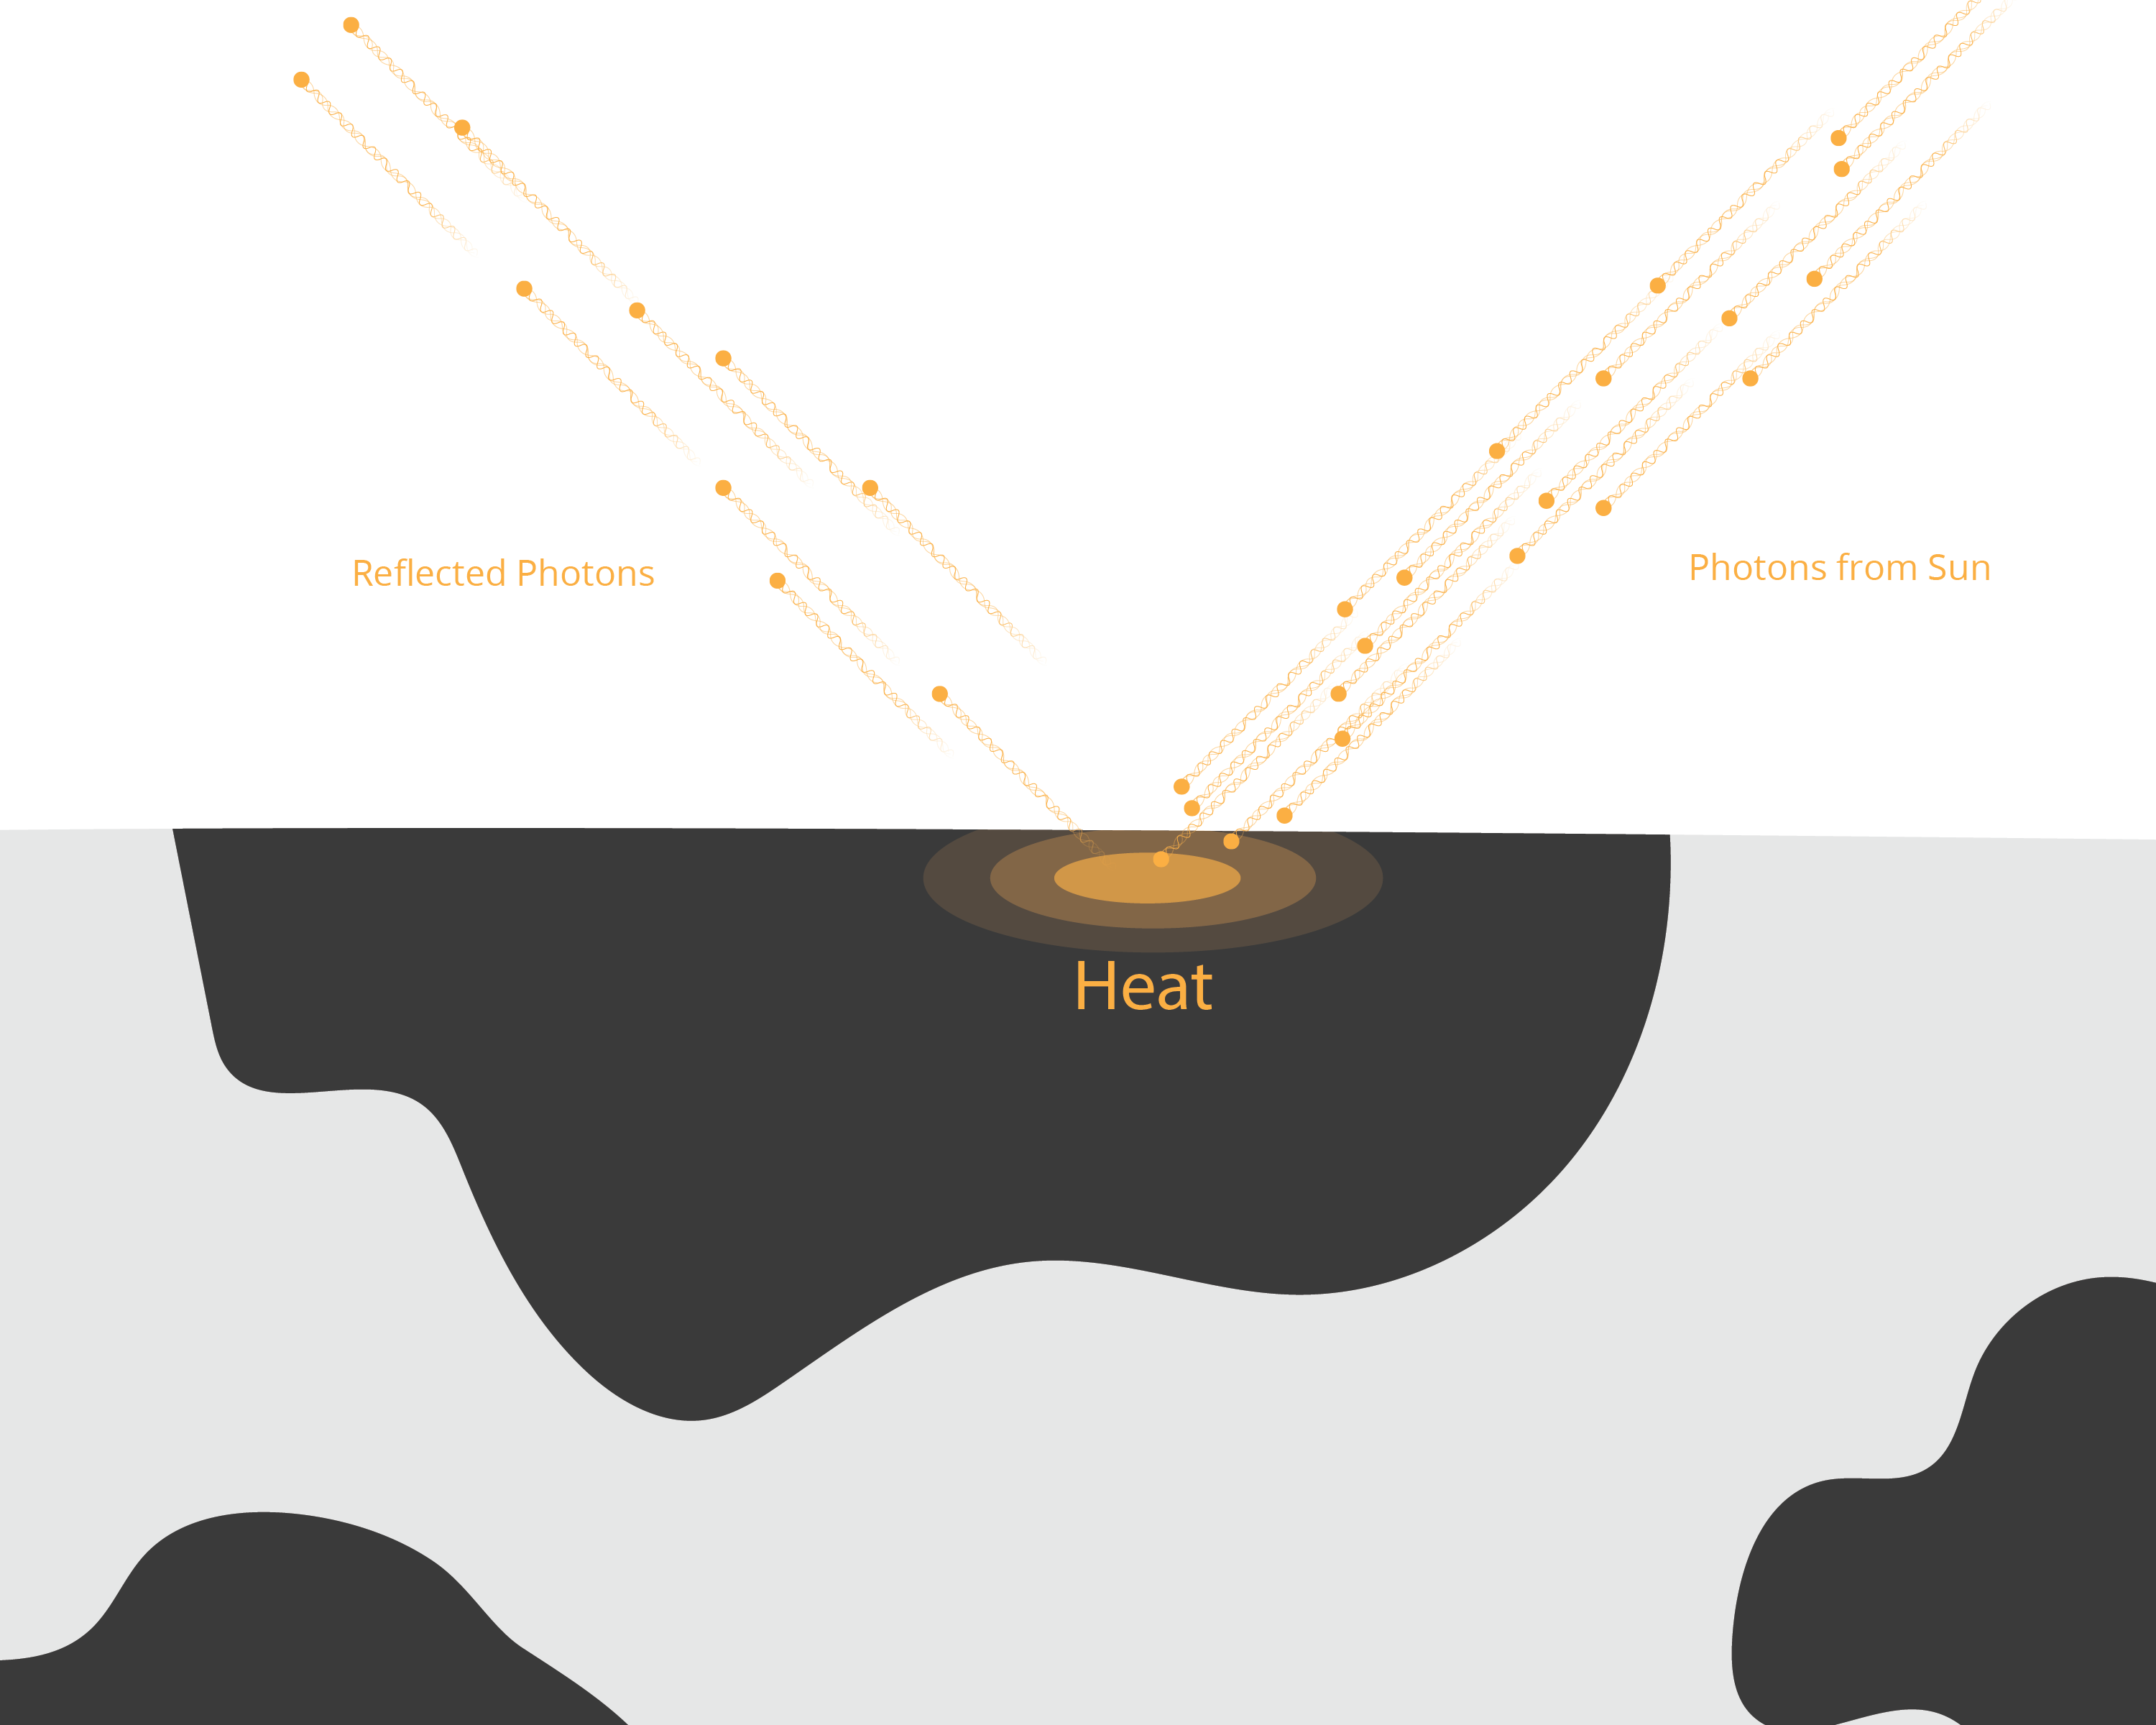
\includegraphics[width=1\textwidth]{cow4.png}
    \caption{Photons hitting the cow create a heated spot, where some are absorbed.}
    \label{fig:example}
\end{figure}
\index{photon!colors of}
\index{photon!wavelength}
Different materials absorb different amounts of each wavelength. A
plant, for example, absorbs a large percentage of all blue and red
photons that hit it, but it absorbs only a small percentage of the
green photons that hit it. Thus, we say ``That plant is green.''

White things absorb very small percentages of photons of any visible
wavelength. Black things absorb very \emph{large} percentages of
photons of any visible wavelength. That is why, on a hot summer day, a black car with black 
seats and interior will heat up on the inside much hotter than a white car. 

Before we go on, let's review: The sun creates photons that travel as
electromagnetic waves of assorted wavelengths to the cow. Many of
those photons are absorbed, but some are not. Some of those photons
that are not absorbed go into the lens of our camera.

\section{Pinhole camera}
\index{camera ! pinhole}
The simplest cameras have no lenses. They are just a box. The box has
a tiny hole that allows photons to enter. The side of the box
opposite the hole is flat and covered with film or some other
photo-sensitive material.

The photons entering the box continue in the same direction they were
going when they passed through the hole. Thus, the photons that
entered from high hit the back wall at a low point. The photons that came from
the left hit the back wall on the right. This is how the image is projected
onto the back wall, rotated 180 degrees; what was up is down, what was
on the left is on the right.
\begin{figure}[htbp]
    \centering
    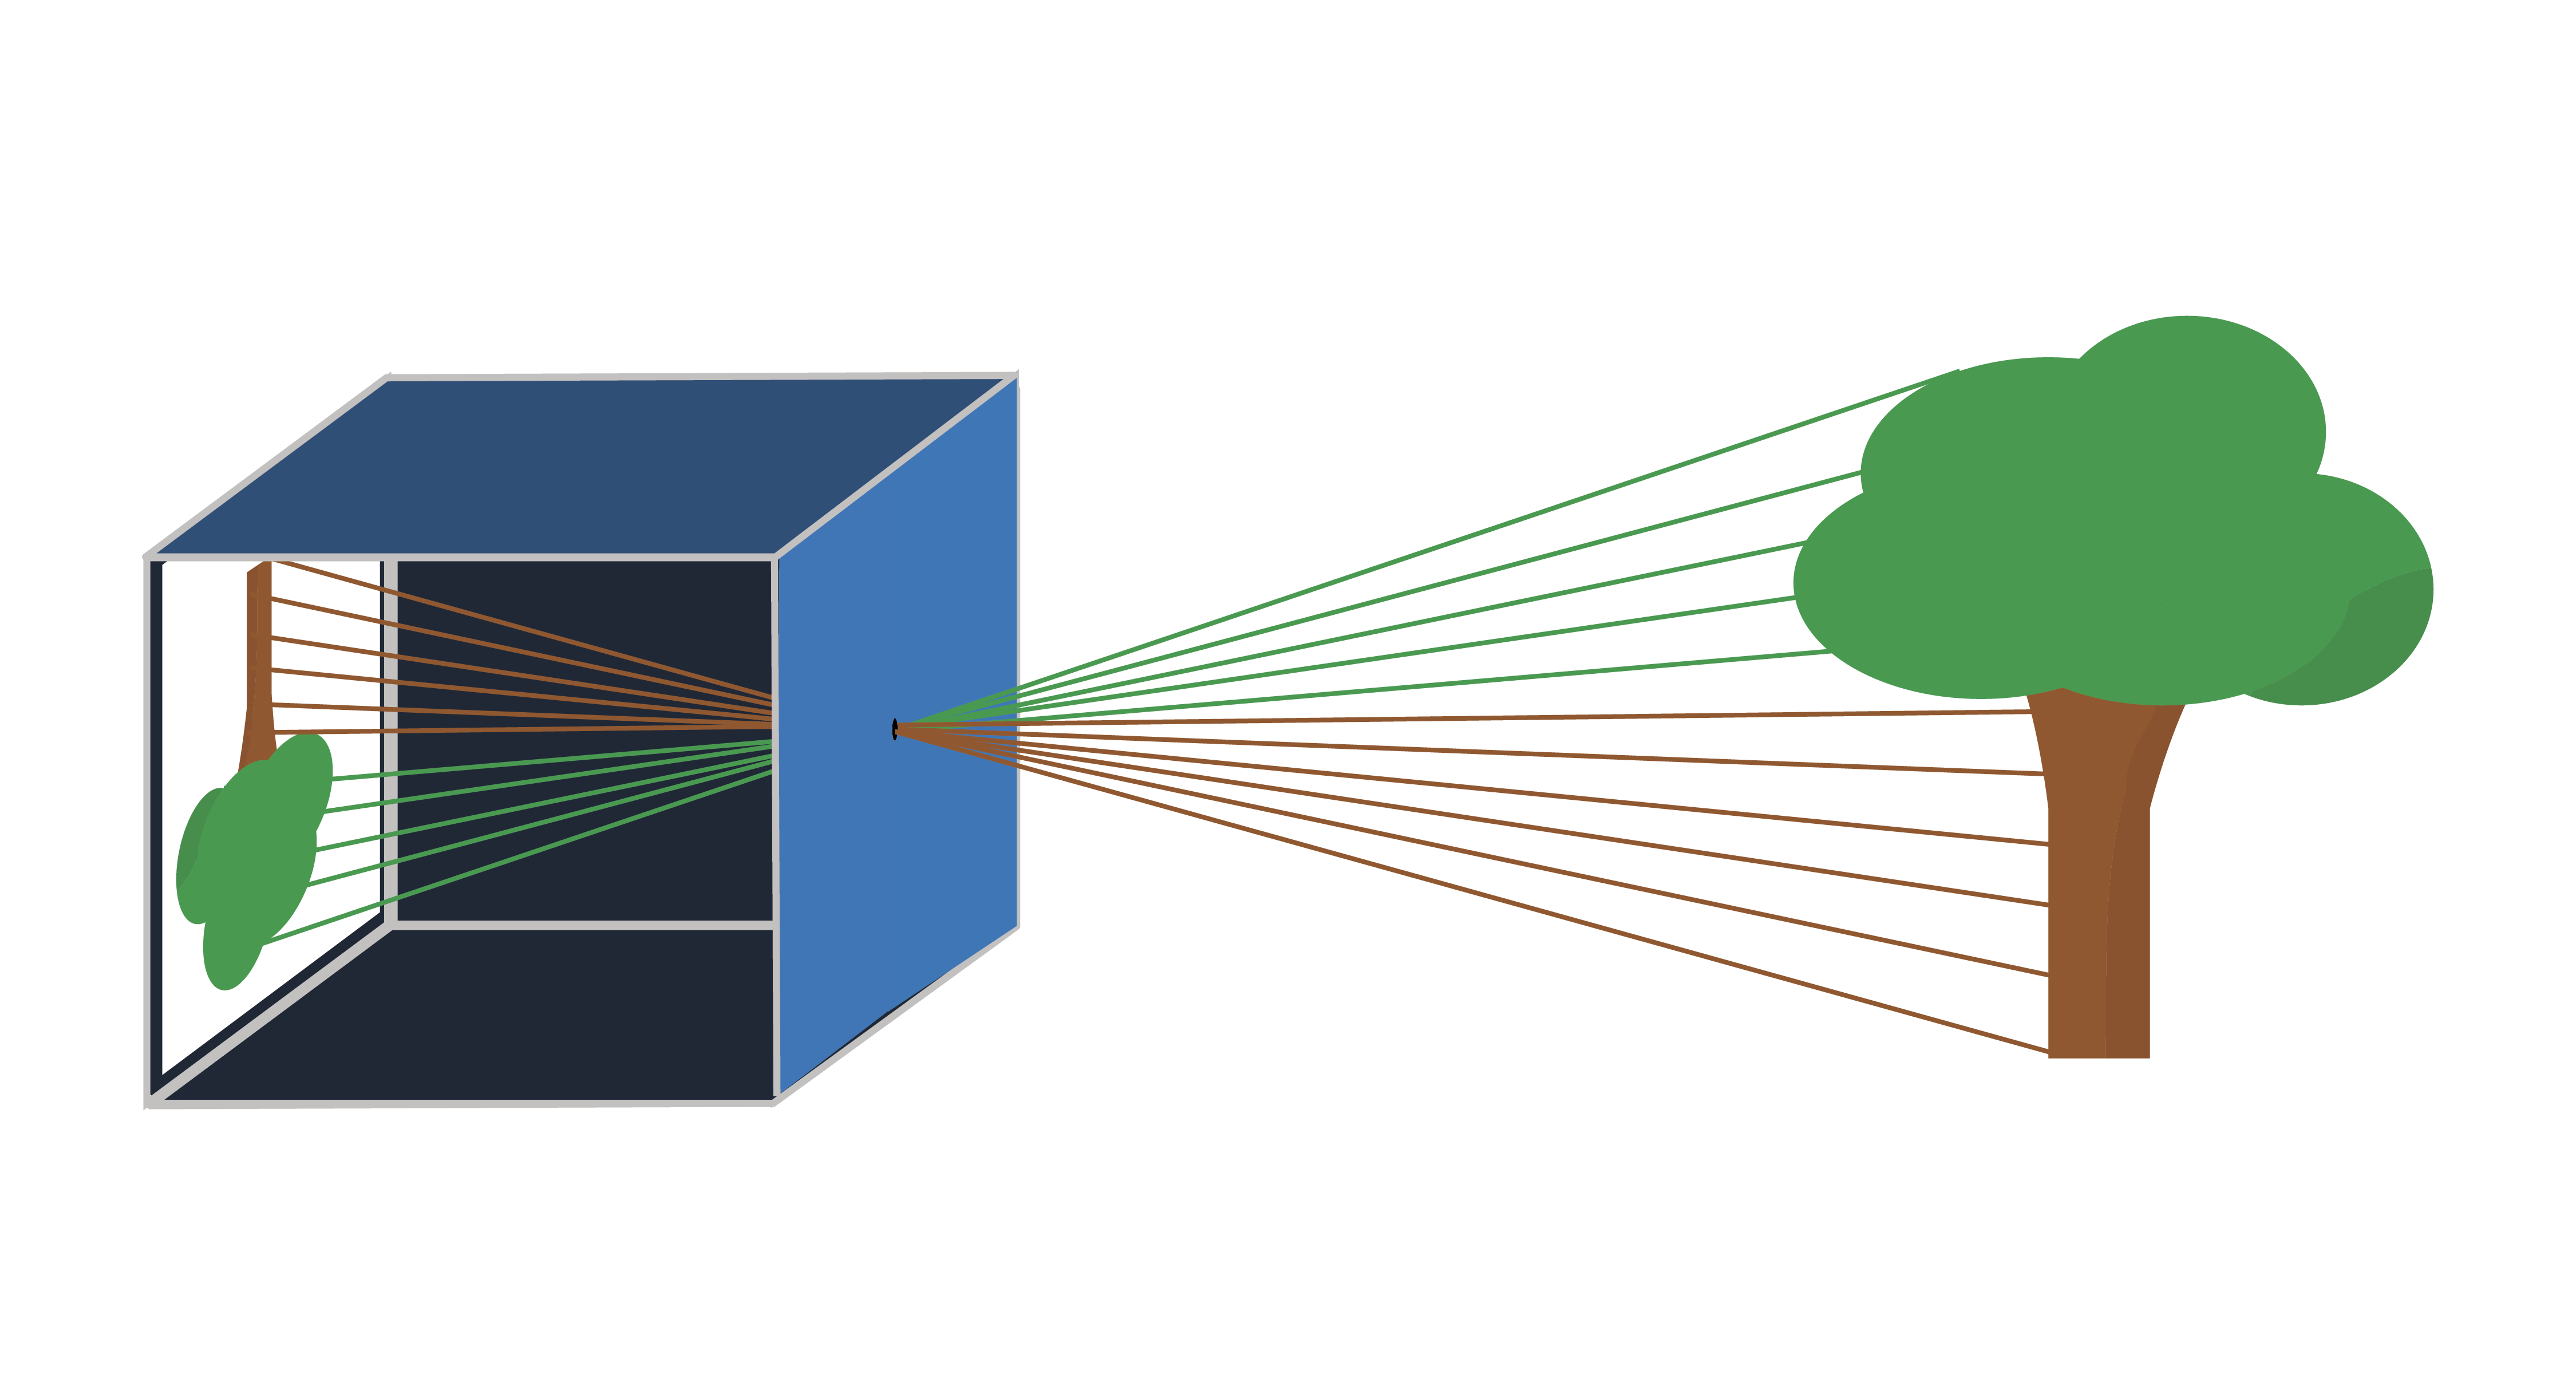
\includegraphics[width=1\textwidth]{pinholeCamera.png}
    \caption{A pinhole camera flips the image it ``sees'' by 180$^\circ$.}
    \label{fig:example}
\end{figure}


\begin{Exercise}[title={Height of the image}, label=image_height]

FIXME: cow swap
%FIXME diagram ^
Let's say that that the pinhole is exactly the same height as the
shoulder of the cow, and that the shoulder is directly above one hoof.
This means the pinhole, the shoulder, and the hoof form a right triangle.

Now, let's say that the camera is being held perpendicular to the
ground. The pinhole, the image of the shoulder, and the image of
the hoof on the back wall of the camera now also form a right triangle.

These two triangles are similar.

The shoulder is 2 meters from the hoof. The cow is standing 3 meters
from the camera. The distance from the pinhole to the back wall of
the camera is 3 cm. How tall is the image of the cow on the back wall
of the camera?

\end{Exercise}
\begin{Answer}[ref=image_height]

The two triangles are similar; one is 2 m and 3m, the other is $x$ cm and 3 cm.

The image of the cow is 2 cm tall.

\end{Answer}

\section{Lenses}

Now, a quick review: A photon leaves the sun in some random direction. It
travels 150 million km from the sun and hits a cow. It is not
absorbed by the cow, and heads off in a new direction. It passes
through the pinhole and hits the back wall of the camera. That seems
incredibly improbable, right?

It actually is relatively improbable, especially if there isn't a lot of
light --- like you are taking the picture at dusk. To increase the
odds, we added a \newterm{lens} to the camera.
\index{camera ! lens}
If you focus a lens on a wall and you draw a dot on that
wall, the lens is designed such that all the photons from the dot that
hit the lens get redirected to the same spot on the back wall of the
camera --- regardless of which path it took to get to the lens.
\begin{figure}[htbp]
    \centering
    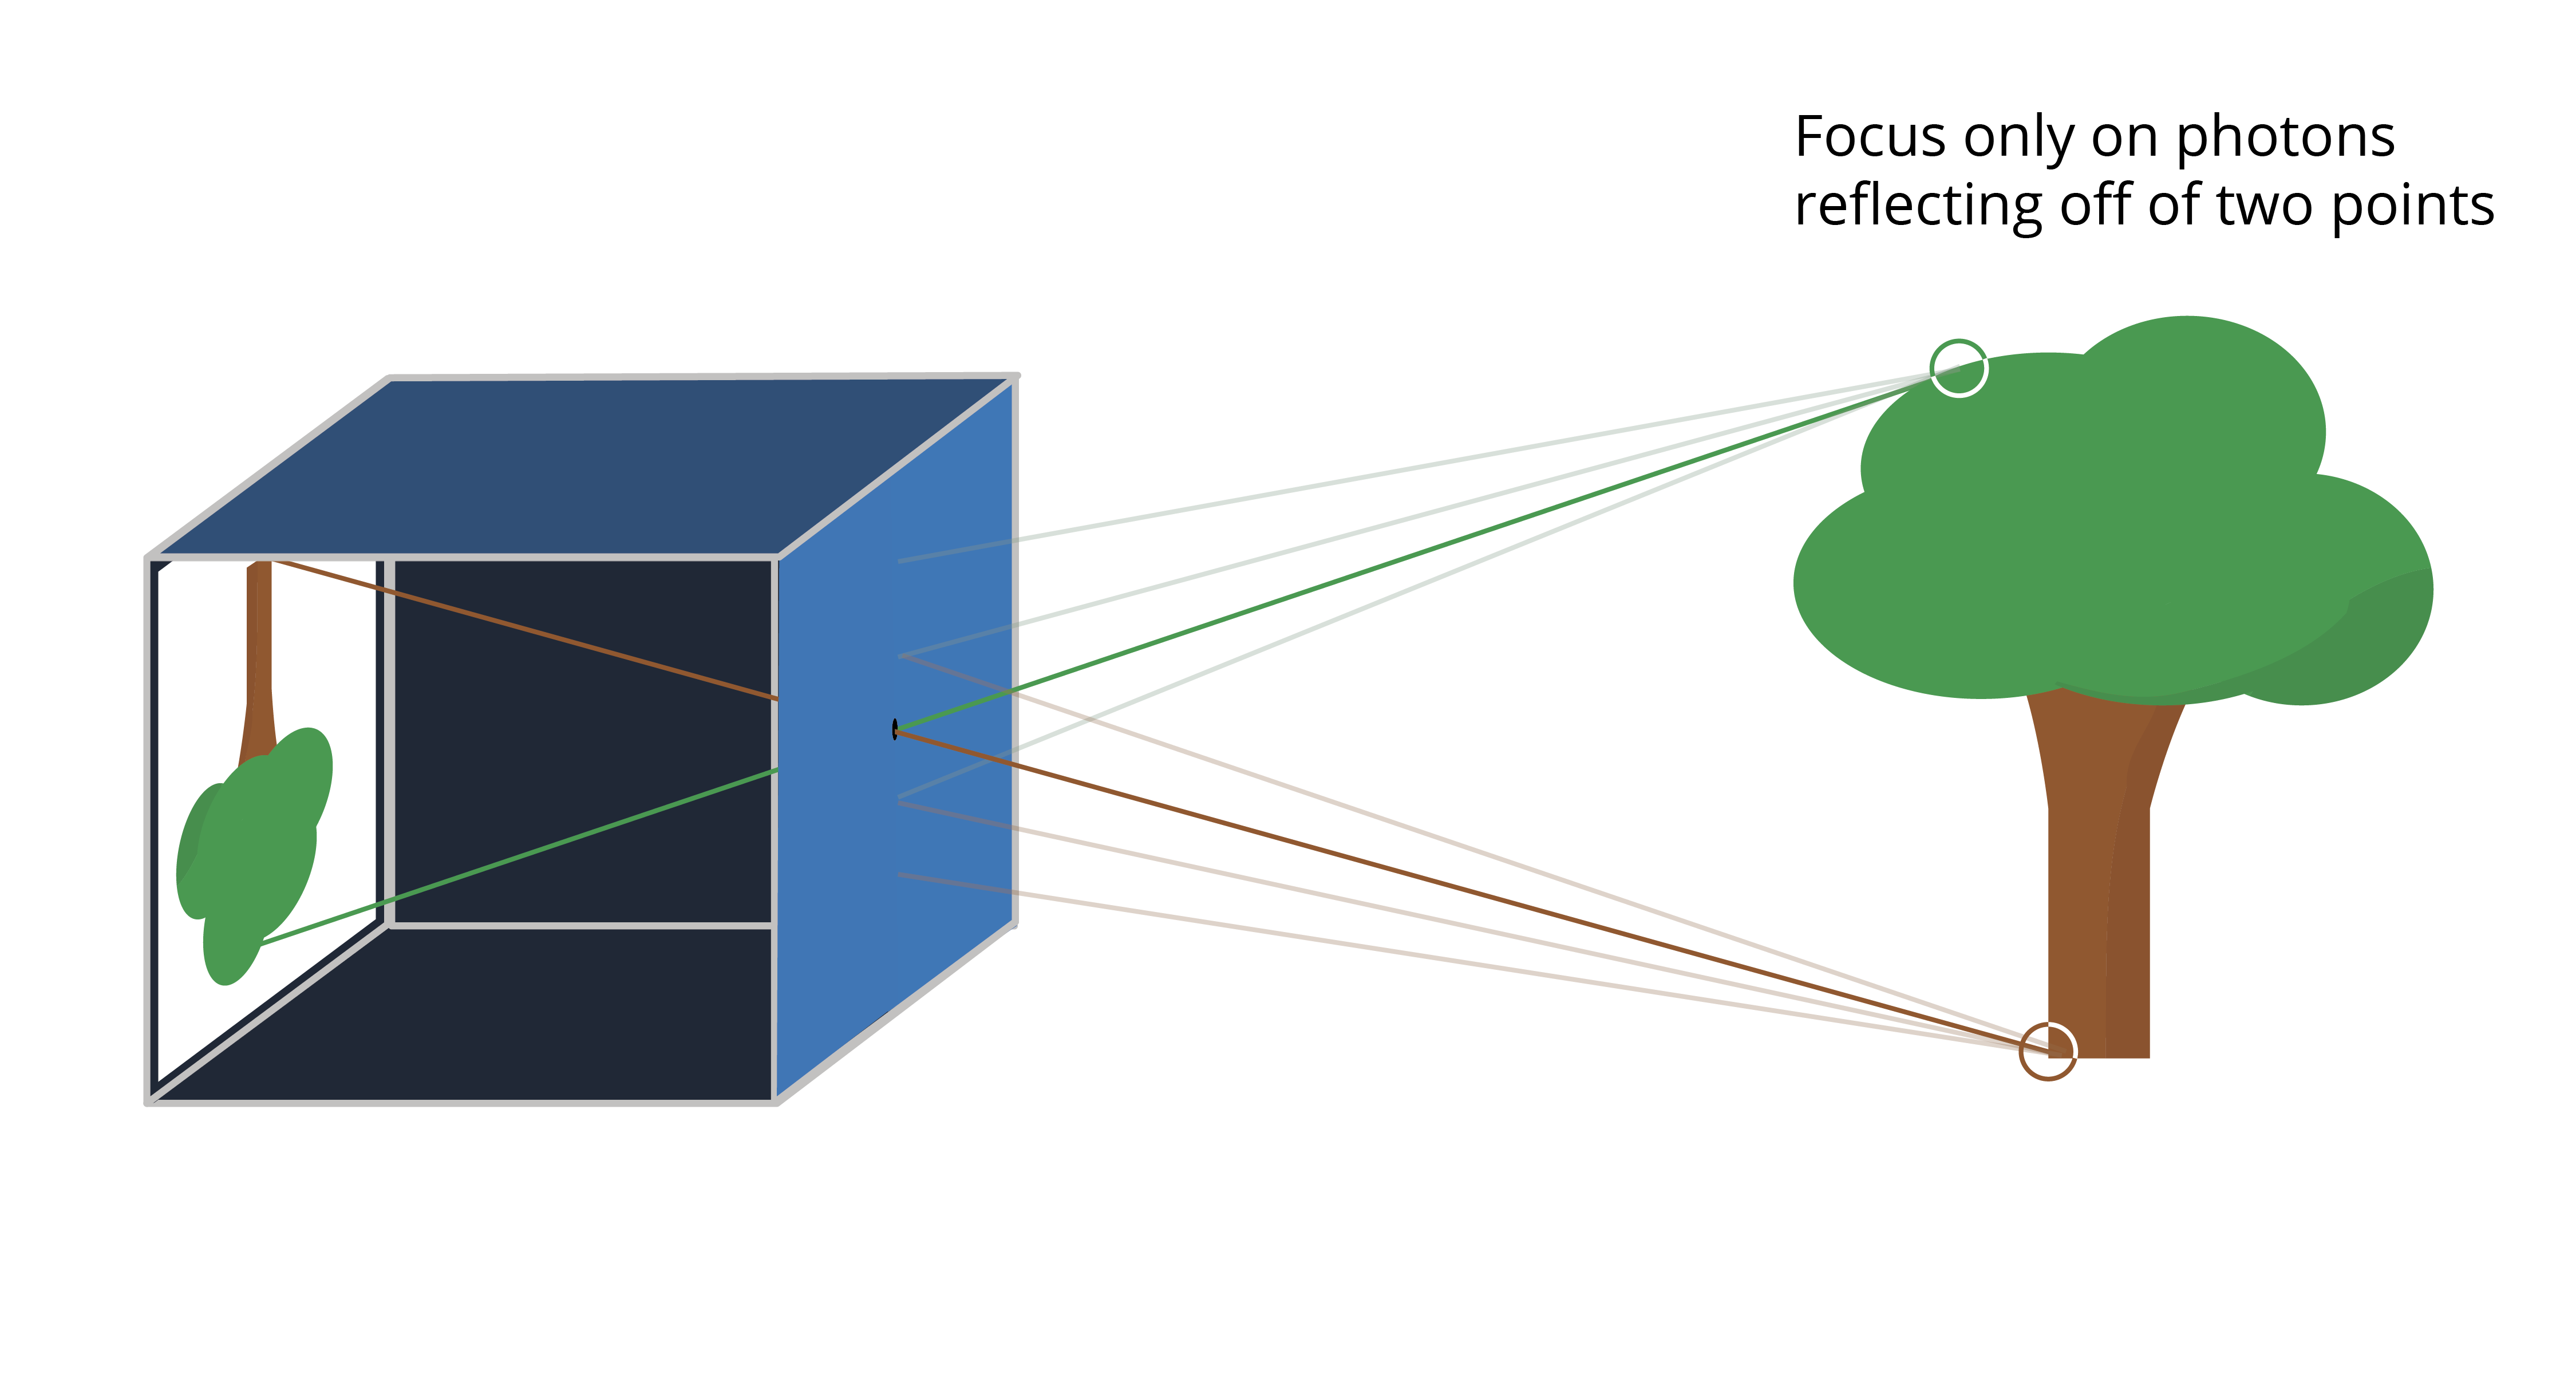
\includegraphics[width=1\textwidth]{pinholePoints.png}
    \caption{A pinhole with a lens allows you to choose the points it reflects.}
    \label{fig:pinholePoints}
\end{figure}



Note that the image still gets flipped. There is a \newterm{focal
point} that all the photons pass through.
\begin{figure}[htbp]
    \centering
    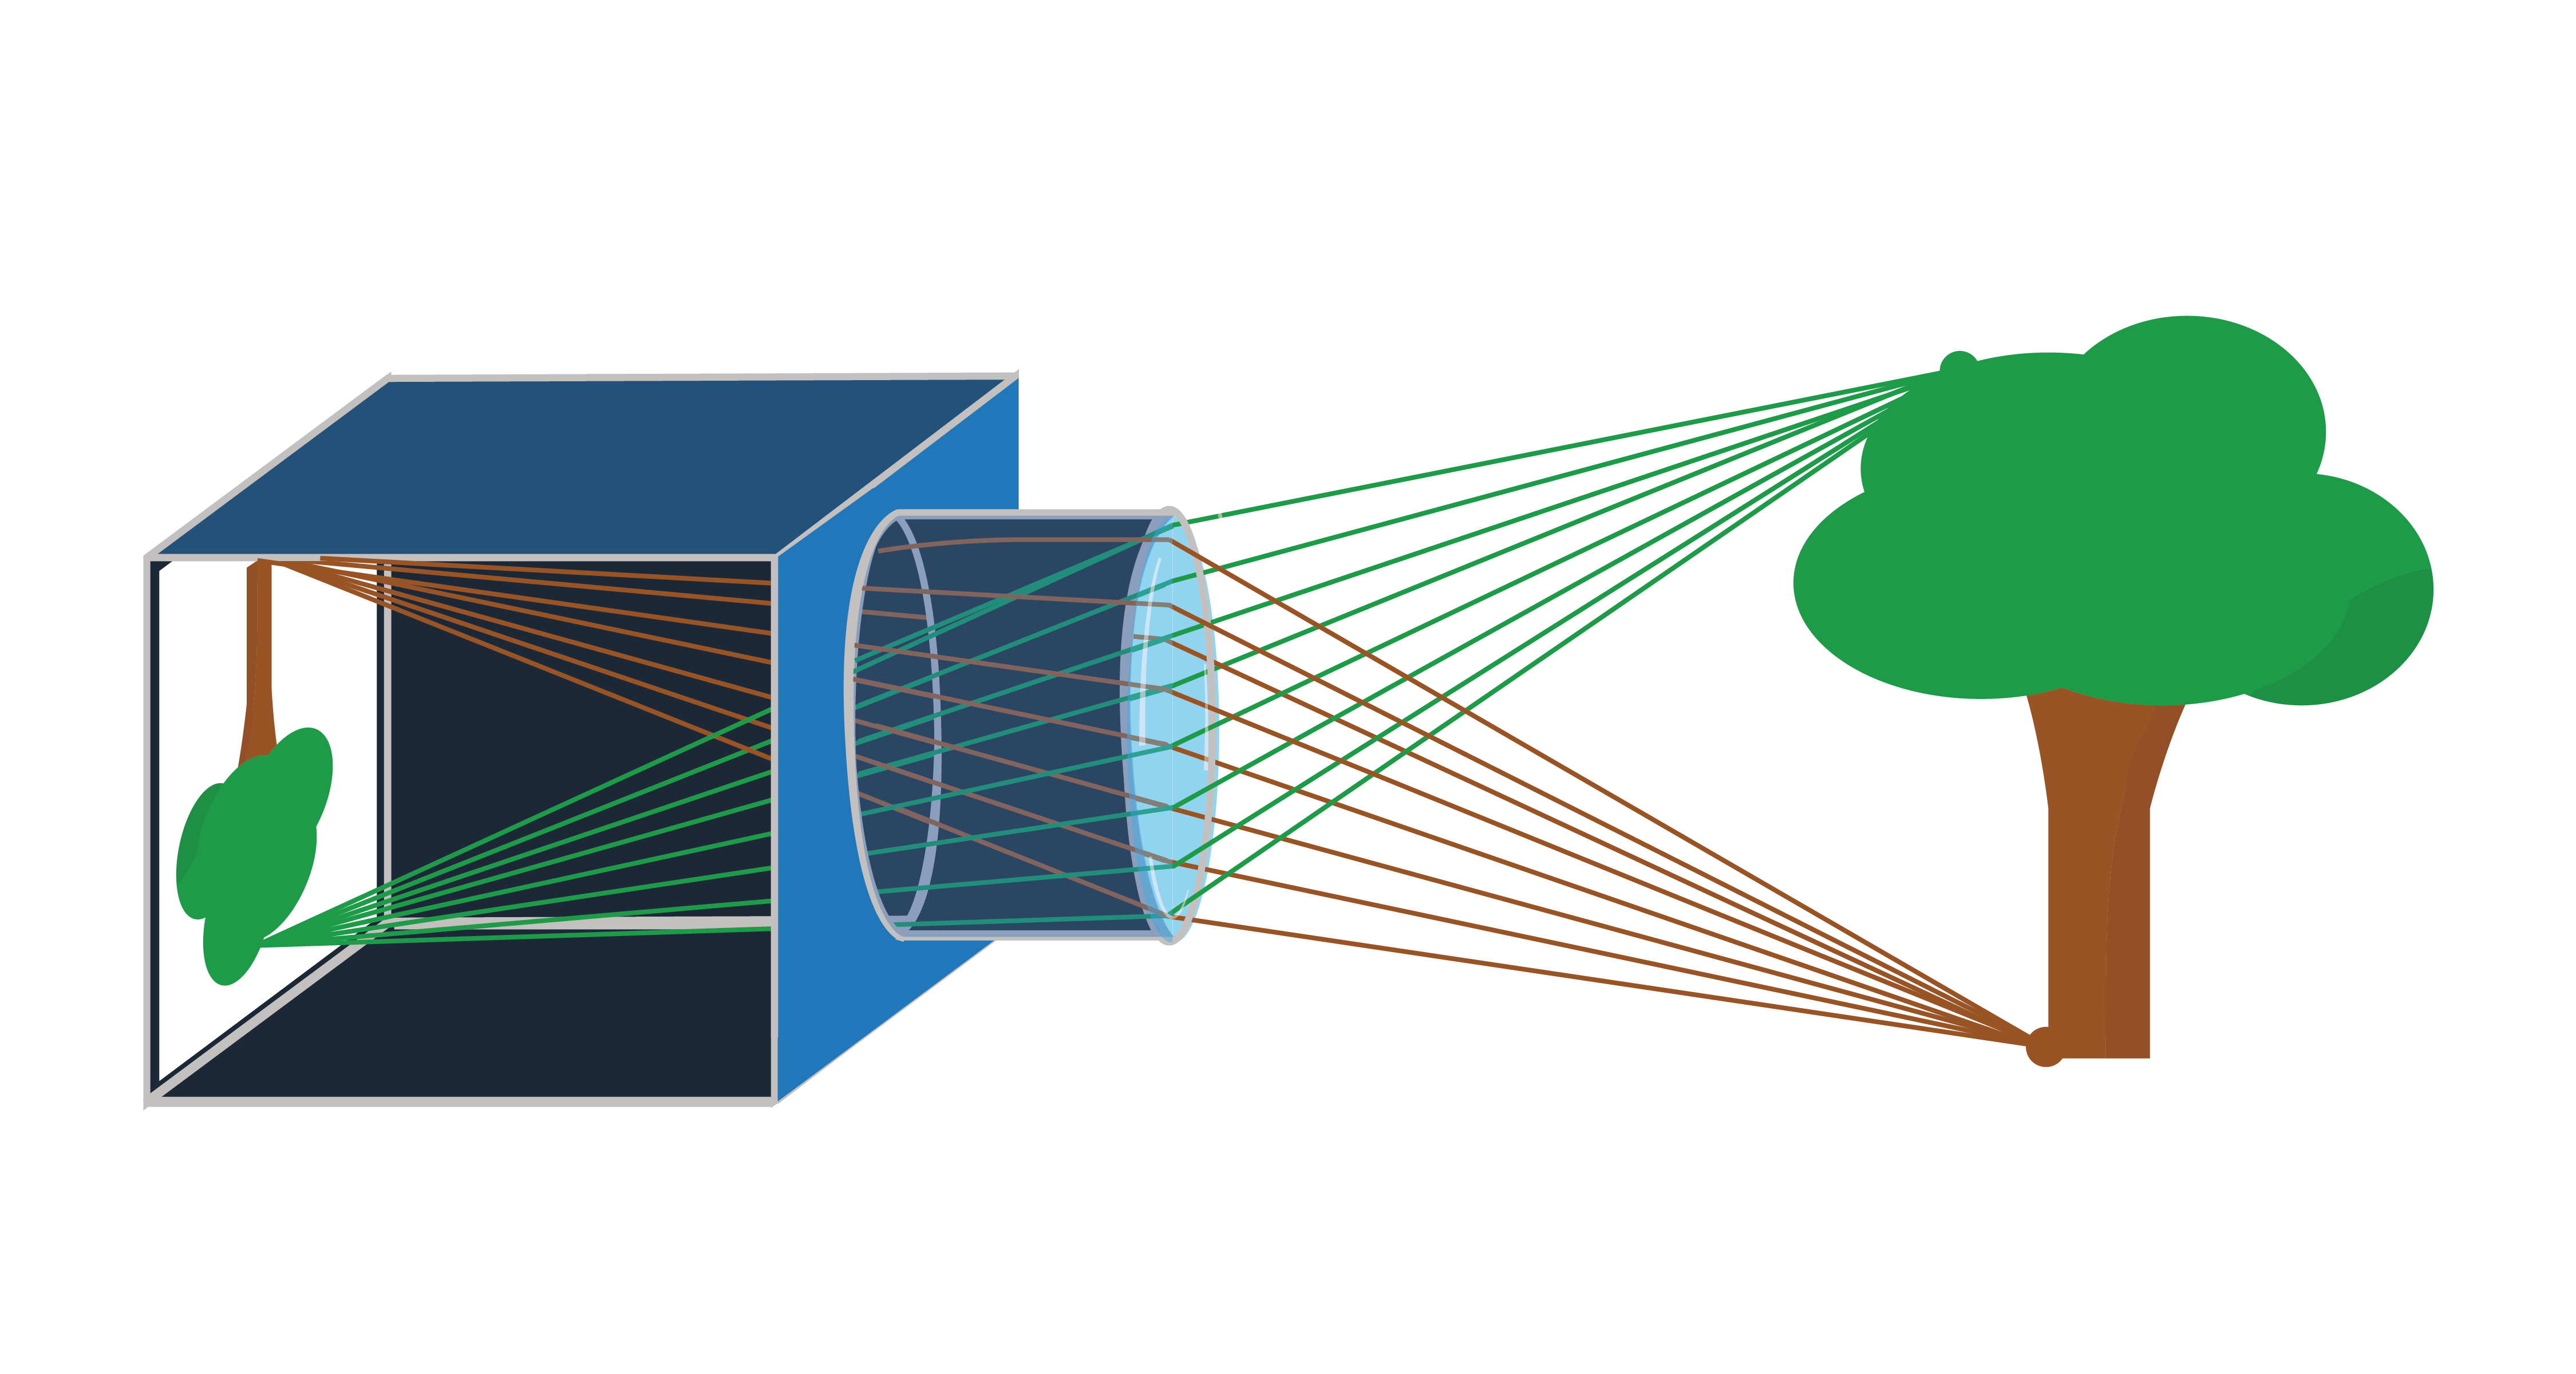
\includegraphics[width=1\textwidth]{lensPoints.png}
    \caption{A lens still flips the image, but introduces a focal point.}
    \label{fig:lensPoints}
\end{figure}

The distance from the lens to its focal point is called the lens's
\newterm{focal length}.\index{camera ! lens ! focal length} Telephoto lenses, that let you take big
pictures of things that are far away, have long focal lengths.
Wide-angle lenses have short focal lengths.
% fixme insert of micro vs macro lenses
% https://electronics.sony.com/imaging/lenses/all-e-mount/p/sel600f40gm
% https://www.amazon.com/Canon-50mm-1-8-STM-Lens/dp/B00X8MRBCW/ref=sr_1_6?dib=eyJ2IjoiMSJ9.yWi0YgvJDa9tyKYiV3H3e7SYBgWhAQqSmxmyaUjpkDmJKzk-MrDdGfBpCZ8QI9WvbyA86tzNWWeXvmnXb-ottilZo7ZMd2iZGgCtyogJxHxpydJyA-sDDj8qrag8SiNU9gcuPriWYjLzQALVSJYy_-ywDIoZEvH8_SXA8JhlbPnjWnp-SUWKvedzrNGJKdlDXU2bQezhoXMamg7vHUc5hH1r30aYIMYgh2Eajc7ugUE.LtorAWasOYMMwoOBej_dSLXbbqiomQXCAhsQueyVr-Q&dib_tag=se&keywords=canon%2Bmacro%2Blens&qid=1754077739&sr=8-6&th=1

\section{Sensors}

The camera on your phone has a sensor on the back wall of the
camera. The sensor is broken up into tiny rectangular regions called
pixels. When you say a sensor is 6000 by 4000 pixels (most common ratio for photography), we are saying
the sensor is a grid of 24,000,000 pixels: 6000 pixels wide and
4000 pixels tall.

Each pixel has three types of cavities that take in photos. One of the
cavities measures the amount of short wavelength light, like blues and
violets. One of the cavities measures the long wavelength light, like
reds and oranges. One of the cavities measures the intensity of
wavelengths in the middle, like greens.
\index{rgb}
Thus, if your camera has a resolution of $6000 \times 4000$, the image
is 72,000,000 numbers: Every one of the 24,000,000 pixels yeilds three
numbers: intensity of long wavelength, mid wavelength, and short
wavelength light. We call these numbers ``RGB'' for Red, Green, and
Blue. The RGB values range from $0-255$ for each channel. We will talk more about this when hexidecimal is introduced.  
% https://en.wikipedia.org/wiki/RGB_color_model#Numeric_representations
% FIXME expand this to introduce hex pixel values?

% \section{Aspect Ratio}
% FIXME
% some quiz questions use this. 